\documentclass[implementacija.tex]{subfiles}
\usepackage{subfiles}
\documentclass[12pt,oneside]{memoir} 
\usepackage[latinica]{matfmaster} 

\begin{document}
K\^{o}d svake Android aplikacije je podeljen u dva direktorijuma: \textbf{app} i \textbf{src}. Osnovnu strukturu \textbf{app} direktorijuma bilo koje Android aplikacije čine poddirektorijumi: 

\begin{itemize}
\item \textit{build} sa izvršnom verzijom koda,
\item \textit{libs} sa eksternim bibliotekama odnosno bibliotekama koje nisu deo Androida, Java ili Kotlin programskih jezika i
\item \textit{src} sa izvornim kodom.
\end{itemize}

 Direktorijum \textbf{src} se uglavnom sastoji od sledećih poddiretkorijuma: 
\begin{itemize}
\item \textit{AndroidTest} u kom se smeštaju svi testovi koje je potrebno pokrenuti na Android uređaju, 
\item \textit{test} u kom se smeštaju svi testovi za testiranje jedinica koda (eng. \textit{unit tests})
\item \textit{main} u kom se nalazi ceo izvorni k\^{o}d.
\end{itemize}

Projekat implementacije upravljača za digitalnu televiziju je smešten u direktorijumu pod nazivom \textit{RemoteControlApp}. Srž aplikacije se nalazi u \textbf{main} poddirektorijumu, a za ovu aplikaciju ovaj direktorijum ima sledeću strukturu:
\begin{itemize}
\item \textit{AndroidMainifest.xml} --- datoteka koji opisuje glavne postavke aplikacije,
\item \textit{res} --- direktorijum sa svim XML datotekama koje čine korisnički interfejs (eng. \textit{user interface}) aplikacije,
\item \textit{java} --- direktorijum sa svim klasama i interfejsima aplikacije
\item \textit{proto} --- direktorijum sa \textit{.proto} datotekama koje su neophodne za korišćenje \textit{Google Cloud API}-ja.
\end{itemize}

\section{Upravljanje procesom izdgradnje i određivanje zavisnosti aplikacije}

Važne datoteke pri postavljanju projekta su \textbf{\textit{build.gradle}} datoteke koje služe da  upravljaju procesom izgradnje i odrede zavisnosti (eng. \textit{dependency}) aplikacije. Ove datoteke se generišu automatski pri kreiranju projekta, ali je moguće dodati sve dodatne zavisnosti koje budu potrebne. Postoje dva tipa ovih datoteka --- na nivou projekta i na nivou modula. Datoteku na nivou projekta čini skup pravila koji važi za ceo projekat, dok datoteke na nivou modula čine pravila za modul u kom se nalazi datoteka. Svaka ova datoteka se sastoji od vise blokova koji grupišu unutar sebe pravila, odnosno opcije koje se primenjuju.

Za uspešno korišćenje \textit{Google Cloud} servisa u aplikaciji, neophodno je uvesti podršku za obradu \textit{Protobuf} (skraćeno od eng. \textit{Protocol Buffers}) datoteka. \textit{Protobuf} je interfejs za definiciju jezika (eng. \textit{Interface Definition Language}, skraćeno IDL) koji definiše strukturu podataka i programski interfejs. \cite{sajt:protobuf} Omogućava usaglašeost pri deljenju struktuiranih podataka između različitih sistemskih platformi i jezika programiranja. Neophodno je unutar bloka \textit{plugins} dodati dodatak \verb|id 'com.google.protobuf'| kako bi se obezbedila adekvatna podrška. Takođe u okviru bloka \textit{protobuf}, se dodaju opcije za korišćenje protobuf-a. Tačne zavisnosti koje je potrebno dodati biće navedene kod opisa implementacije glasovnih komandi gde će biti i objašnjena povezanost \textit{Google cloud} servisa i \textit{protobuf}-a.

\section{Potrebne dozvole i informacije za pokretanje aplikacije}

Informacije potrebne za pokretanje i instalaciju aplikacije čine datoteku \textit{AndroidManifest.xml}. U ovoj datoteci su definisane sve dozvole koje aplikacija zahteva od uređaja sa kog se pokreće aplikacija: pristup internetu, stanju bežične mreže (eng. \textit{WiFi}), stanju telefona, vibracija i  snimanje audio sadržaja. Pregled ovih dozvola je dat u listingu \ref{lst:manifestApp}. Kao što je navedeno u delu \ref{sec:manifest} glavna etiketa koja mora postojati je za aplikaciju i u okviru nje su postavljene vrednosti naziva aplikacije, slika kojom je aplikacija predstavljena, ciljani API nivo kao i dve aktivnosti koje se pojavljuju. Prva aktivnost je \textit{ChooseConnection}, koja je odabir uređaja sa kojim će se korisnik povezati i ona je obeležena kao glavna aktivnost. Druga aktivnost je \textit{RemoteView} koja čini prikaz daljinskog upravljača. 

\lstinputlisting[language=XML, caption= {Odobrenja definisana u datoteci \textit{AndroidManifest.xml}}, label={lst:manifestApp}]{implementacije/kodovi/AppManifest.xml}


\section{Resursi aplikacije}
Direktorijum u kom se smeštaju svi resursi aplikacije se naziva \textit{res}. Resursi koji se mogu čuvati su slike, planovi (eng. \textit{layout}), stringovi, stilovi itd. Moguće je čuvati iste resurse u različitim dimenzijama kako bi u zavisnosti od dimenzija i podešavanja uređaja bili odabrani odgovarajući resursi. Direktorijum \textit{drawable} skladišti slike. Za potrebe projekta formirane su i sačuvane slike za strelicu koja je predstavljena trouglom, ovalno dugme i dugme za prekid konekcije. 

Vrednosti, boje i dimenzije za različite resurse se skladište u direktorijumu \textit{values}. Datoteka \textit{colors.xml} sadrži boje korišćene za kreiranje interfejsa. Stringovi potrebni za dizajn korisničkog interfejsa su sačuvani u \textit{strings.xml}. Kolor shema, odnosno tema aplikacije je definisana u \textit{themes/themes.xml} odakle se može uočiti da boje koje se koriste za korisnički interfejs su nijanse plave boje. 

Svaki ekran sa kojim se korisnik može susresti mora imati korisnički interfejs koji ima svoj plan opisan unutar XML datoteke. Skup svih planova je smešten unutar direktorijuma \textit{layout} koji kod ove aplikacije ima sledeće XML datoteke:
\begin{description}
\item[\textbf{activity\_choose\_stb}] predstavlja plan ekrana za odabir konekcije, odnosno stb uređaja sa kojim korisnik želi da se poveže. Ovaj plan je kreiran pomoću klase \textit{RelativeLayout}. Unutar \textit{RelativeLayout}-a nalaze se tri komponente koje se mogu prikazati ili skloniti u zavisnosti od potrebe. Prva komponenta je \textit{RecyclerView} sa id-jem \textit{@+id/rv\_boxes\_list} sa podešenom vidljivošću na \textit{gone} što znači da je inicijalno skriven. Njegova vidljivost se menja u kodu u trenutku kada se pronađu uređaji na mreži tako što se postavlja na \textit{visible}, odnosno da je vidljiv. Sledeća komponenta je \textit{ProgressBar} koji može poslužiti prilikom učitavanja. Poslednja komponenta je \textit{RelativeLayout} sa id-jem \textit{@+id/rl\_pairing\_container} koji je inicijalno sakriven. On sadrži tekstualno polje tipa \textit{TextView} sa uputstvom korisniku da unese k\^{o}d koji vidi na ekranu uređaja sa kojim pokušava uparivanje, polje za unos teksta tipa \textit{EditText} u koji se unosi k\^{o}d i dugme za potvrdu unosa. Ceo prikaz za uparivanje postaće vidljiv kada korisnik odabere uređaj sa kojim želi da se poveže. Prikaz ovih elemenata je pokriven u opisu rada aplikacije.

\item[\textbf{remote\_control\_scene}] predstavlja izgled daljinskog upravljača. Sve komponente su unutar \textit{ConstraintLayout}-a koji omogućava da udaljenost komponenti bude predstavljena ograničenjima (eng. \textit{constraint}). Ovakvo predstavljanje kompontenti olakšava prilagođavanje prikaza ekrana na uređajima različitih dimenzija. Korisnički interfejs ovog plana kao i shematski plan zajedno sa svim ograničenjima se može videti na slici \ref{fig:remoteScena}. Dugmići za kontrolu uključenosti uređaja, prekid konekcije sa povezanim uređajem, vraćanje nazad, gašenje zvuka i mikrofoni su objekti tipa \textit{ImageButton}. Svi ostali dugmići su kreirani pomoću klase \textit{Button}. Nad svim dugmićima je postavljena opcija da se na pritisak dugmeta pozove metoda \textit{onClick()}. O akcijama koje se dese prilikom pritiska dugmeta i poziva metode \textit{onClick} biće reči u nastavku poglavlja. U prvom nizu su dugmići za paljenje/gašenje uređaja, zatim dugme \textit{GUIDE} koje prikazuje elektronski vodič kroz program (eng. \textit{Electronic Program Guide (EPG)}) i na kraju dugme za prekid konekcije između uređaja. Dugmići za brojeve su podeljeni u četiri horizontalna \textit{LinearLayout}-a sa po tri dugmeta. Poslednji od njih sadrži i dugme \textit{MOVIE} koje prikazuje obabir filmova za iznajmljivanje i dugme \textit{LIVE} koje prebacuje ekran na sadržaj koji je uživo na tv-u. Centralni deo ekrana zauzima dugme za potvrdu izbora \textit{OK} i strelice za levo, desno, gore i dole. Strelice su kreirane samostalno i u implementaciji je zato potrebno dodati  \verb|android:background="@drawable/arrow"|. Dugmići za povratak na prethodno prikazano, mikrofoni i \textit{HOME} - prikaz početnog ekrana su grupisani u jedan \textit{LinearLayout}. Na samom dnu ekrana se nalazi još jedan \textit{LinearLayout} koji se sastoji od dva vertikalna \textit{LinearLayout}-a, za menjanje kanala i podešavanje jačine zvuka. Između njih je dugme za totalno gašenje zvuka.

\item[\textbf{stb\_view}] je jedan \textit{RelativeLayout} koji čini samo jedan \textit{TextView}. On se ubacuje unutar \textit{RecyclerView}-a kada je potrebno prikazazi pronađene uređaje. Predstavlja ime jednog uređaja koji je pronađen. Inicijalno nema nikakav tekst.
\end{description}

%=================== SLIKA ======================================
\begin{figure}[!ht]
  \centering
  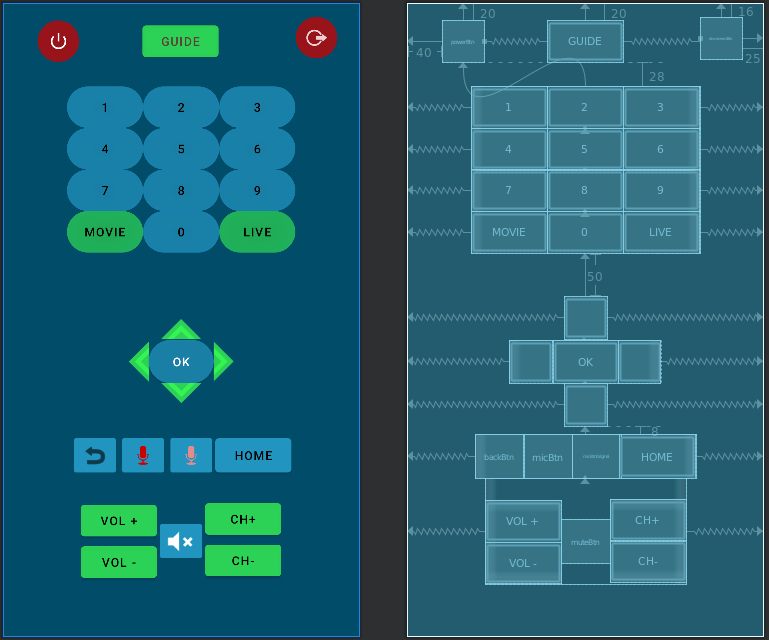
\includegraphics[width=\textwidth]{Implementacija/snimci_ekrana/remote_control_scene.png}
  \caption{Korisnički interfejs i shematski plan daljinskog upravljača}
  \label{fig:remoteScena}
\end{figure}
%=====================================================================

% opisati sve ove fajlove koje imam

\section{Struktura direktorijuma java}
Za funkcionisanje aplikacije neophodno je da se omogući pronalaženje uređaja, a zatim i da se manipuliše sa odabranim uređajem. Kako bi ovo sve radilo ispravno potrebna je međusobna interakcija između klasa, kao i podela koda u adekvatne pakete i klase prema funkcionalnostima koje obezbeđuju. Iz tih razloga unutar glavnog paketa aplikacije k\^{o}d je podeljen u dva paketa. Paket \textbf{stbs} sadrži klase koje se bave pronalaženjem i upravljanjem STB uređajem. Klase koje se bave upravljanjem komandama i komunikacijom sa uređajem su smeštene u paket \textbf{controller}.  Dijagram paketa je prikazan na slici XXXXXXXXXXXX

Klase unutar paketa \textbf{stbs} su:
\begin{itemize}
\item \textit{ChooseAdapter} koja se koristi za prikaz liste pronađenih uređaja,
\item \textit{ChooseConnection} koja se koristi za odabir i povezivanje sa izabranim uređajem,
\item \textit{DiscoveryHandler} se koristi za pronalaženje dostupnih uređaja na mreži,
\item \textit{NsdDiscover} koja se koristi za korišćenje NSD (eng. \textit{Network Service Discovery}) mehanizma za pronalaženje uređaja i
\item \textit{Stb} koja predstavlja jedan uređaj i sadrži informacije o njemu.
\end{itemize}
Dijagram klasa ovog paketa se može videti na slici XXXXXXXXX.

Klase unutar paketa \textbf{controller} su:
\begin{itemize}
\item \textit{CommandsHandler} koja je odgovorna za obradu i slanje komandi na uređaj,
\item \textit{RemoteView} koja se bavi prikazom daljinskog upravljača i interakcijom korisnika sa aplikacijom,
\item \textit{UdpClient} koja omogućava komunikaciju putem UDP protokola i
\item \textit{StreamingRecognizeClient} koje se koristi za obradu audio podataka i prepoznavanje govora pomoću \textit{Google Cloud API}-ja. 
\end{itemize}
Komunikacija i izgled ovih klasa su prikazani na dijagramu XXXXXXXXX.

Pored ovih klasa u glavnom paketu aplikacjie nalaze se sledeće klase i interfejsi:
\begin{itemize}
\item \textit{AsyncDataReceiver} interfejs služi za primanje asinhronih podataka,
\item \textit{AsyncReceiver} interfejs služi za primanje asinhronih podataka,
\item \textit{OnItemClickedListener} interfejs služi za obradu klikova na elemente liste,
\item \textit{Singleton} klasa se koristi za implementaciju Singlton (eng. \textit{Singleton}) šablona i
\item \textit{Constants} klasa koja skladišti sve konstante potrebne u razvoju aplikacije.
\end{itemize}
NJihov dijagram klasa je prikazan na slici XXXXXXXXXXX.

\section{Implementacija glavnih funkcionalnosti aplikacije}
Kao što je navedeno u delu \ref{opis_rada} postoje koraci koji su potrebni da se ispune kako bi se aplikacija koristila za upravljanje uređajem za digitalnu televiju. U nastavku će biti prikazani delovi koda i objašnjenja kako implementirati pretragu uređaja na mreži, povezivanje sa odabranim uređajem kao i komunikaciju i slanje komandi na uređaj. Poseban osvrt će biti na implementaciji zadavanja glasovnih komandi. 

\subsection{Implementacija pretrage uređaja}
\subfile{implementacije/impl_pretraga}


\subsection{Implementacija povezivanja sa odabranim uređajem}
\subfile{implementacije/impl_povezivanje}

\subsection{Implementacija komunikacije sa uređajem i zadavanja komandi}
\subfile{implementacije/impl_komunikacija}


\subsection{Implementacija zadavanja glasovnih komandi}
% \subfile{}

\section{Direktorijum proto}



% slika podele koda src -> Manifets, res, com, proto + gradle
% Manifest sta ima, glavni delovi
% gradle kako je podesen
% res folder, ukratko xml implementacije neki specif. stvari
% com folder -> tu imamo 2 paketa + ovi glavni
% proto kad i zasto je koriscen
\end{document}